%!TEX root = ./main.tex

%%**************************************************************
%%
%% DHBW Heidenheim - Template for Bachelor Thesis
%%
%% Bevor usisng this template please have a look at the REAMDME.md file
%%
%%**************************************************************

%!TEX root = ../main.tex

% show warning for old LaTeX syntax
\RequirePackage[l2tabu, orthodox]{nag}

\documentclass[
	pdftex,
	oneside,  
	12pt,			    % fontsize
	parskip=half,		    % Space (in lines) between paragraphs
	headheight = 12pt,    % Header hight
	headsepline,		    % Line after header
	footheight = 16pt,	    % Footer height
	footsepline,		    % Line before footer
	abstracton,		    % Abstract headline
	DIV=calc,		    % Calculate print space
	BCOR=8mm,		    % BCOR settings (Bindekorrektur)
	headinclude=false,   % Exclude header from print space
	footinclude=false,	    % Exclude footer from print space
	listof=totoc,		    % Show List of Figures/Tables in Contents
	toc=bibliography,	    % Show Bibliography in Contents
]{scrreprt}	                     % Koma-Script report-class, long document: scrreprt, short document: scrbook

\usepackage{xstring}
\usepackage[utf8]{inputenc}
\usepackage[T1]{fontenc}

% iflang command definition
\newcommand{\iflang}[2]{%
  \IfStrEq{\documentLanguage}{#1}{#2}{}%
}

% ifDocType comand definition
\newcommand{\ifDocType}[3]{%
  \IfStrEq{\documentType}{#1}{#2}{#3}%
}

% ifMultipleAuthors definition
\newcommand{\ifMultipleAuthors}[2]{%
  \IfStrEq{\multipleAuthors}{true}{#1}{#2}%
}

% ifSpecialDocument definition
\newcommand{\ifSpecialDocument}[2]{\IfStrEqCase{\documentType}{%
	{T2_1000}{#2\ignorespaces}%
	{T2\_2000}{#2\ignorespaces}%
	{T2\_3100}{#2\ignorespaces}%
	{T2\_3300}{#2\ignorespaces}%
	}[#1\ignorespaces]%
}

% Include main settings
%!TEX root = ../main.tex

%% Citation Styles
% http://ctan.mirrorcatalogs.com/macros/latex/contrib/biblatex/doc/biblatex.pdf (3.3.1 Citation Styles)
% recommended:  z.B numeric-comp, alphabetic, 
% not recommended: authoryear, alphabetic-verb, 
\newcommand{\quoteStyle}{alphabetic-verb}

%% Fonts
%% palatino, goudysans, lmodern or libertine
\newcommand{\documentFont}{lmodern}

%% Margin
\newcommand{\margin}{2.5cm}

%% Space between chapter headline and top of page
\newcommand{\chapterMargin}{20pt}

%% Table settings
% Column spacing
\newcommand{\tableColumnMargin}{10pt}
%Line spacing
\newcommand{\tableRowMargin}{1.5}

%% Color settings
\newcommand{\defineColors}{%
	\definecolor{LinkColor}{HTML}{\linkColor}
	\definecolor{ListingBackground}{HTML}{F8F8F8}
}

%% Syntax Highlighting (Listings)
\newcommand{\listingsettings}{%
	\lstset{%
		language=Java,			% default language
		numbers=left,			% position of line numbers (left, right)
		stepnumber=1,			% set number to each line
		numbersep=5pt,			% 5pt between number and source code
		numberstyle=\tiny,		% letter size of numbers
		breaklines=true,		        % break lines if necessary (true, false)
		breakautoindent=true,	        % indenting after break line (true, false)
		postbreak=\space,		% break line after space
		tabsize=2,				% tabulator size
		basicstyle=\ttfamily\footnotesize, % font style
		showspaces=false,		% show space (true, false)		showstringspaces=false,	% show space in strings (true, false)
		extendedchars=true,		% show all Latin1 characters (true, false)
		captionpos=b,			% sets the caption-position to bottom
		backgroundcolor=\color{ListingBackground}, % source code background
		xleftmargin=10pt,		        % margin left
		xrightmargin=5pt,		        % margin right
		frame=single,			        % border settings
		frameround=ffff,
		rulecolor=\color{darkgray},	% border color
		fillcolor=\color{ListingBackground},
		aboveskip=20pt,
		keywordstyle=\color[rgb]{0.133,0.133,0.6},
		commentstyle=\color[rgb]{0.133,0.545,0.133},
		stringstyle=\color[rgb]{0.627,0.126,0.941},
		numberbychapter=true
	}
}
 

% Include document settings
%!TEX root = ../main.tex

%% Document language (en, de)
\newcommand{\documentLanguage}{de}

%% Document type
% T2\_1000 Project Thesis (Semester 1 & 2)
% T2\_2000 Project Thesis (Semester 3 & 4)
% T2\_3100 Seminar Paper (Semester 5 & 6)
% T2\_3300 Bachelor Thesis
\newcommand{\documentType}{T2\_2000}

\newcommand{\multipleAuthors}{false}
\newcommand{\documentAuthor}{Sarah Hägele}
\newcommand{\documentTitle}{Konzeptionierung und Implementierung einer automatischen Testdatengenerierung für ein System zur Integration externer Massendaten}
\newcommand{\documentPeriod}{24 Wochen}

\newcommand{\matriculationNumber}{9596606}

\newcommand{\locationUniversity}{Heidenheim}
\newcommand{\department}{Informatik}
\newcommand{\course}{TINF2020AI}

\newcommand{\degree}{Bachelor of Science}
% INF2014 - INF2016 (MI):       Bachelor of Science
% INF2014 - INF2016 (IA/IM) :   Bachelor of Engineering
% INF2017 (all):                Bachelor of Science

% A lecture that the document is written for
\newcommand{\lecture}{Software Engineering}
% Whether to show the lecture on cover
\newcommand{\showLecture}{false}

\newcommand{\releaseDate}{Juni 2022}
\newcommand{\releaseLocation}{Heidenheim}

\newcommand{\companyName}{FNT GmbH}
\newcommand{\companyLocation}{Ellwangen}

\newcommand{\tutor}{Dipl.-Ing.~(FH) Marcus Fetzer}
%\newcommand{\evaluator}{Prof. Dr.\ Rolf Assfalg}

\newcommand{\linkColor}{00007A}


% Load language specific Strings
\input{lang/\documentLanguage}

% Load language specific babel package
\iflang{de}{\usepackage[english, ngerman]{babel}}
\iflang{en}{\usepackage[ngerman, english]{babel}} 

% Add comment feature
\newcommand{\comment}[1]{\par {\bfseries \color{blue} #1 \par}}


%%%%%%% Package Includes %%%%%%%

\usepackage[margin=\margin,foot=1cm]{geometry}
\usepackage[activate]{microtype}                                         
\usepackage[onehalfspacing]{setspace}
\usepackage{makeidx}
\usepackage[autostyle=true,german=quotes]{csquotes}
\usepackage{longtable}
\usepackage{enumitem}	                                                 
\usepackage{graphicx}
\usepackage{pdfpages}                                                         
\usepackage{xcolor} 	                                                    
\usepackage{float}
\usepackage{array}
\usepackage{calc}		                         
\usepackage[right]{eurosym}
\usepackage{wrapfig}
\usepackage{pgffor}                                                             
\usepackage[perpage, hang, multiple, stable]{footmisc}  
\usepackage[printonlyused]{acronym}                                 
\usepackage{listings}
\usepackage[obeyFinal,backgroundcolor=yellow,linecolor=black]{todonotes}
\usepackage{rotating}
\usepackage{lscape}
\usepackage{amsmath}
\usepackage{amssymb}
\usepackage{\documentFont}
\usepackage[%
	pdftitle={\documentTitle},
	pdfauthor={\documentAuthor},
	pdfsubject={\documentType},
	pdfcreator={pdflatex, LaTeX with KOMA-Script},
	pdfpagemode=UseOutlines,       % Show Contents while opening
	pdfdisplaydoctitle=true, 		% Show document title instead of file name
	pdflang={\documentLanguage}, % Document language
]{hyperref}
\usepackage{bookmark}
\usepackage[nonumberlist,toc]{glossaries}

% Generate glossary
\makeglossaries{}

% Load colors
\defineColors{}

% Set Titel, Autor and Date
\title{\documentTitle}
\author{\documentAuthor}
\date{\datum}


% PDF link settings
\hypersetup{%
	colorlinks=true, 		
	linkcolor=LinkColor, 	
	citecolor=LinkColor,
	filecolor=LinkColor,
	menucolor=LinkColor,
	urlcolor=LinkColor,
	linktocpage=true, 
	bookmarksnumbered=true 
}

% Captions fontsize
\addtokomafont{caption}{\small}

% Bibliographie settings
\iflang{de}{%
\usepackage[
	backend=biber,		% recommended. Alternative: bibtex
	bibwarn=true,
	bibencoding=utf8,	         % If .bib file is encoded with utf8, otherwise ascii
	sortlocale=de_DE,
	style=\quoteStyle,
]{biblatex}
}
\iflang{en}{%
\usepackage[
	backend=biber,		% recommended. Alternative: bibtex
	bibwarn=true,
	bibencoding=utf8,        % If .bib file is encoded with utf8, otherwise ascii
	sortlocale=en_US,
	style=\quoteStyle,
]{biblatex}
}

\addbibresource{bibliographie.bib}

% Hurenkinder und Schusterjungen verhindern
% http://projekte.dante.de/DanteFAQ/Silbentrennung
\clubpenalty = 10000 % schließt Schusterjungen aus (Seitenumbruch nach der ersten Zeile eines neuen Absatzes)
\widowpenalty = 10000 % schließt Hurenkinder aus (die letzte Zeile eines Absatzes steht auf einer neuen Seite)
\displaywidowpenalty=10000

% Graphicspath
\graphicspath{{images/}}

% frequently used programing languages
\lstloadlanguages{PHP,Python,Java,C,C++,bash}

\listingsettings{}
% Rename Listings
\renewcommand\lstlistingname{\listingPhrase}
\renewcommand\lstlistlistingname{\listListingPhrase}
\def\lstlistingautorefname{\authorListingPhrase}
\lstdefinestyle{myLangStyleB}{
  literate={\{}{{\CodeSymbol{\{}}}1
           {[}{{\CodeSymbol{[}}}1, 
}

% Spaces in tables
\setlength{\tabcolsep}{\tableColumnMargin}
\renewcommand{\arraystretch}{\tableRowMargin}

\definecolor{groovyblue}{HTML}{0000A0}
\definecolor{groovygreen}{HTML}{008000}
\definecolor{darkgray}{rgb}{.4,.4,.4}
\colorlet{punct}{red!60!black}
\definecolor{background}{HTML}{EEEEEE}
\definecolor{delim}{RGB}{20,105,176}
\colorlet{numb}{magenta!60!black}
 
\lstdefinelanguage{Groovy}[]{Java}{
  keywordstyle=\color{groovyblue}\bfseries,
  stringstyle=\color{groovygreen}\ttfamily,
  keywords=[3]{each, findAll, groupBy, collect, inject, eachWithIndex},
  morekeywords={def, as, in, use},
  moredelim=[is][\textcolor{darkgray}]{\%\%}{\%\%},
  moredelim=[il][\textcolor{darkgray}]{§§}
}

\lstdefinelanguage{json}{
    showstringspaces=false,
    literate=
     *{:}{{{\color{punct}{:}}}}{1}
      {,}{{{\color{punct}{,}}}}{1}
      {\{}{{{\color{delim}{\{}}}}{1}
      {\}}{{{\color{delim}{\}}}}}{1}
      {[}{{{\color{delim}{[}}}}{1}
      {]}{{{\color{delim}{]}}}}{1},
	  morestring=[b]"
}


\input{content/glossary}

\begin{document}

	% Cover
	\begin{spacing}{1}
		%!TEX root = ../main.tex

\begin{titlepage}
	\begin{longtable}{p{8cm} p{8cm}}
		\raggedright {\raisebox{\ht\strutbox-\totalheight}{\includegraphics[height=2.5cm]{images/cover/logo-dhbw.pdf}}} &
		% no company logo for semester paper and special documents
		\ifDocType{T2\_3100}{}{%
			\ifSpecialDocument{}{%
				\raggedleft {\raisebox{\ht\strutbox-\totalheight}{
\includegraphics[height=2.5cm]{images/cover/fnt-company-logo.png}}}
			}%
		}%
	\end{longtable}
	\enlargethispage{20mm}
	\begin{center}
		\doublespacing{
		\vspace*{12mm}	{\LARGE\textbf \documentTitle }}\\
		\vspace*{12mm}	{\large\textbf {\documentTypePhrase}}\\
		
		% degre only for bachelor thesis
		\ifDocType{T2\_3300}{
			\vspace*{12mm}	\degreePhrase\\
			\vspace*{3mm}		{\textbf \degree}\\
		}

		\IfStrEq{\showLecture}{true}{
			\vspace*{12mm}	\lecturePhrase\\
			\vspace*{0mm}		{\textbf \lecture}\\
		}

		\vspace*{12mm}	\departmentPhrase{} \department\\
    \vspace*{0mm}		\locationUniversityPhrase{} \locationUniversity\\
		\vspace*{12mm}	\documentAuthorPhrase\\
		\vspace*{3mm}		{\large\textbf \documentAuthor}\\
		\vspace*{12mm}	\releaseDate\\
	\end{center}
	\vfill
	\begin{spacing}{1.2}
	\begin{tabbing}
		mmmmmmmmmmmmmmmmmmmmmmmmmm             \= \kill
		\textbf{\documentPeriodPhrase}       \>  \documentPeriod\\
		\textbf{\matriculationNumberPhrase, \coursePhrase}  \>  \matriculationNumber, \course\\

		% no company for the semester paper and special documents
		\ifDocType{T2\_3100}{}{%
			\ifSpecialDocument{}{%
				\textbf{\companyPhrase}                  \>  \companyName, \companyLocation\\
			}%
		}%
		\textbf{\tutorPhrase}               \>  \tutor\\

		% evaluator only for bachelor thesis
		\ifDocType{T2\_3300}{%
			\textbf{\evaluatorPhrase}              \>  \evaluator
		}{}
	\end{tabbing}
	\end{spacing}
\end{titlepage}

	\end{spacing}
	\newpage

	\pagenumbering{Roman}

	% Restriction notices
	\ifDocType{T2\_3100}{%
		% no restricition notices for semester paper
	}{%
		\input{ads/restrictionNotices}
		\newpage
	}%

	% Declaration
	\input{ads/declaration}
	\newpage

	% Abstract
	%!TEX root = ../main.tex

\pagestyle{empty}

% override abstract headline
\renewcommand{\abstractname}{Abstract}

\begin{abstract}
Das ausgiebige Testen ist essentiell zur Entwicklung qualitativ hochwertiger Software. Insbesondere automatisiertes Testen hilft dabei, Testzyklen häufiger durchlaufen zu können und so kleinere Codeänderungen direkt zu prüfen, sodass Fehler möglichst früh entdeckt werden. Die Flexibilität der automatisierten Tests kommt allerdings an ihre Grenzen, wenn die zugrunde liegenden Testdaten manuell gepflegt werden müssen. Das automatische Generieren dieser Testdaten kann dabei helfen, automatisierte Tests noch flexibler und zuverlässiger zu gestalten.

In dieser Arbeit wird eine automatische Testdatengenerierung für die automatisierten Tests des Command Integration Frameworks, einem System zur Integration externer Massendaten, konzeptioniert und realisiert. Zunächst wird der Ist-Zustand analysiert und dessen Schwächen aufgezeigt. Daraufhin wird ein Konzept zur Umsetzung einer Datengenerierung basierend auf definierten Anforderungen erarbeitet. Dieses wird für einige Anwendungsfälle implementiert und erweitert und anschließend in Hinblick auf die Anforderungen, Ziele und den Implementierungsaufwand evaluiert.

\vspace*{20mm}

Thorough testing is essential to the development of high quality software. Automated testing helps in enabling more frequent test runs so that smaller code changes can be validated immediately and faults can be detected as early as possible. The flexibility of automated tests reaches its limits, however, when the underlying test data has to be maintained manually. Generating test data automatically can help in making automated tests more flexible and reliable.

In this thesis, an automated test data generation for the automated tests of the Command Integration Framework, a system for external mass data integration, is conceptualised and realised. Firstly, the status quo is analysed and its weaknesses are outlined. Secondly, a concept for the realisation of the data generation is created based on defined requirements. This concept is implemented for multiple use cases, extended and finally evaluated in regards to the requirements, goals and the implementation effort.
\end{abstract}
	\newpage

        % only page number in footer
	\pagestyle{plain}
	
	% space bevore chapter headline
	\RedeclareSectionCommand[beforeskip=\chapterMargin]{chapter}

	% Contents
	\begin{spacing}{1.1}
		\begingroup
		
		    % set subchapter depth
			\setcounter{tocdepth}{1}
			
			\tableofcontents
			\clearpage
		\endgroup
	\end{spacing}
	\newpage

	% Acronyms
	\cleardoublepage
    %!TEX root = ../main.tex

\addchap{\acronymsPhrase}

\begin{acronym}[YTMMM]
\setlength{\itemsep}{-\parsep}

\acro{AGPL}{Affero GNU General Public License}
\acro{CIF}{Command Integration Framework}
\acro{SQL}{Structured Query Language}
\acro{NMS}{Network Management System}
\acro{QA}{Quality Assurance (Qualitätssicherung)}
\acro{SUT}{System Under Test}
\acro{GUI}{Graphical User Interface (Grafische Benutzeroberfläche)}
\acro{API}{Application Programming Interface (Programmierschnittstelle)}
\acro{BGE}{Business Gateway Entity}
\acro{OSS}{Open Source Software}
\acro{REST}{Representational State Transfer}
\acro{JSON}{JavaScript Object Notation}
\acro{POJO}{Plain Old Java Object}
\acro{Elid}{Element ID}
\acro{CSV}{Comma Separated Value}
\acro{XML}{Extensible Markup Language}
\acro{CoP}{Community of Practice}
\acro{HTTP}{Hypertext Transfer Protocol}
\acro{E2E}{End-to-End}

\end{acronym}


	% List of Figures
	\cleardoublepage
	\listoffigures

	%List of Tables
	\cleardoublepage
	\listoftables

	% List of Listings
	\cleardoublepage
	\lstlistoflistings
	\cleardoublepage

	\pagenumbering{arabic}
	
	\pagestyle{headings}

	%Content
	\foreach \i in {01,02,03,04,05,06,07,08,09,...,99} {%
		\edef\FileName{content/chapter/\i .tex}%
			\IfFileExists{\FileName}{%
				\input{\FileName}
			}
			{%
%				No chapter available
			}
	}

	\clearpage

	% Bibilography
	\cleardoublepage
	\printbibliography


	
	% Appendix
	\appendix
	% !TeX root = ../main.tex

\addchap{\appendixPhrase}

\section*{A. Expertenbefragung}\label{app:befragung}
Im Zuge der des Projekts der automatischen Testdatengenerierung wurde eine anonyme Befragung von drei professionellen Tester*innen bei \textit{FNT} durchgeführt. Die gestellten Fragen und gegebenen Antworten sind im Folgenden im Originaltext aufgeführt.

\begin{longtable}[H]{| p{.2\textwidth} | p{.7\textwidth} |}
    \hline
    \gray 1) & \gray \textbf{Could you briefly describe what exactly your job is at FNT?} \\ 
    \hline
    \textbf{Tester*in 1} & QA Engineer \\ 
    \hline
    \textbf{Tester*in 2} & QA Automation for API \& GUI tests in Command \\ 
    \hline
    \textbf{Tester*in 3} & I work in the QA doing the test designs, manual test execution and am also
    developing the automated tests for mostly the Requests domain \\ 
    \hline
\end{longtable}

\begin{longtable}[H]{| p{.2\textwidth} | p{.7\textwidth} |}
    \hline
    \gray 2) & \gray \textbf{How important would you say the job of a tester is for the development of high
    quality software?} \\ 
    \hline
    \textbf{Tester*in 1} & When it comes to quality assurance, there are several quality gates that need to
    pass in order to deliver a high quality software. Some of these quality gates are
    fulfilled by developers and other by testers. As testers, we ensure that the
    application works as expected by conducting end-to-end tests. Developer's tests
    do not cover such complex tests that testers do. So in this sense, as testers we are
    executing tests that are as close as possible to what the customer will do and have
    the end user perspective, therefore the tester role is vital to the success of the
    product. \\ 
    \hline
    \textbf{Tester*in 2} & essential and it makes the life of developers much easier because they only need to
    make a rough test of their funcion and the QAs can make a full regression test of
    whatever ese could be affected by a change. \\ 
    \hline
    \textbf{Tester*in 3} & who ever heard of "the rule of ten" knows that it's not only important, because of
    security reasons, but also from a monetary kind of perspective. So pretty important
    I'd say \\ 
    \hline
\end{longtable}

\begin{longtable}[H]{| p{.2\textwidth} | p{.7\textwidth} |}
    \hline
    \gray 3) & \gray \textbf{Are you aware of any incidents when software had major bugs after
    insufficient testing?} \\ 
    \hline
    \textbf{Tester*in 1} & Yes \\ 
    \hline
    \textbf{Tester*in 2} & Yes \\ 
    \hline
    \textbf{Tester*in 3} & No \\ 
    \hline
\end{longtable}

\begin{longtable}[H]{| p{.2\textwidth} | p{.7\textwidth} |}
    \hline
    \gray 4) & \gray \textbf{If yes, please elaborate.} \\ 
    \hline
    \textbf{Tester*in 1} & Customer reported performance issues when trying to place several objects in
    Command. For notification-email service, the customer had a special configuration which was
    not part of the test suite. \\ 
    \hline
    \textbf{Tester*in 2} & Unfortunately this appears sometimes because manual release testing is very time
    consuming for multiple weeks and it is often not possible to make a code freeze at
    the same moment you start testing so some functions changed after an sufficient
    test and there is only a smoke test of the funtionality after changing. \\ 
    \hline
    \textbf{Tester*in 3} & I'm sure there were instances, but nothing springs to my mind currently \\ 
    \hline
\end{longtable}

\begin{longtable}[H]{| p{.2\textwidth} | p{.7\textwidth} |}
    \hline
    \gray 5) & \gray \textbf{Are you aware of any incidents when software had major bugs after sufficient
    testing?} \\ 
    \hline
    \textbf{Tester*in 1} & No \\ 
    \hline
    \textbf{Tester*in 2} & No \\ 
    \hline
    \textbf{Tester*in 3} & No \\ 
    \hline
\end{longtable}

\begin{longtable}[H]{| p{.2\textwidth} | p{.7\textwidth} |}
    \hline
    \gray 6) & \gray \textbf{If yes, please elaborate.} \\ 
    \hline
    \textbf{Tester*in 1} & - \\ 
    \hline
    \textbf{Tester*in 2} & - \\ 
    \hline
    \textbf{Tester*in 3} & I'm sure there were instances, but nothing springs to my mind currently \\ 
    \hline
\end{longtable}

\begin{longtable}[H]{| p{.2\textwidth} | p{.7\textwidth} |}
    \hline
    \gray 7) & \gray \textbf{Approximately how many bugs are found per test run?} \\ 
    \hline
    \textbf{Tester*in 1} & Because automated tests are implemented for the regression suite, the number of
    bugs found per test run is highly dependent on the automation coverage, the area in
    which changes occurred and how often the tests are run. So far, the highest number
    of bugs found per test run was 2 (several tests fail but the root cause was the same
    and it was traced back to 2 bugs which were not caught by manual testing, but by
    the automated tests). There are times when test runs finds no new bugs.
    In our team, each new feature is first tested manually - where we find on average
    10-15 bugs, then it is automated (becomes part of the regression suite). \\ 
    \hline
    \textbf{Tester*in 2} & Around 3 per week, but we are running around 4000 automated tests each night \\ 
    \hline
    \textbf{Tester*in 3} & This really depends for us automated testers if there were any recent changes, so
    there's no definitive number I can tell. But I guess it's around two, when there were
    bigger changes in the code \\ 
    \hline
\end{longtable}

\begin{longtable}[H]{| p{.2\textwidth} | p{.7\textwidth} |}
    \hline
    \gray 8) & \gray \textbf{How important do you consider the test data to be for high quality testing?} \\ 
    \hline
    \textbf{Tester*in 1} & Test data is of great significance for production like scenarios.  \\ 
    \hline
    \textbf{Tester*in 2} & Very, if possible it should be as real and (for automation) constant as possible to
    identify in a fast way if it is reated to the change or data. \\ 
    \hline
    \textbf{Tester*in 3} & Because our test cases are use case driven it surely is better/important to work with
    data that is as close as possible to the data that our users will use. \\ 
    \hline
\end{longtable}

\begin{longtable}[H]{| p{.2\textwidth} | p{.7\textwidth} |}
    \hline
    \gray 9) & \gray \textbf{How does it work to create test data for new tests and new test instances of
    software?} \\ 
    \hline
    \textbf{Tester*in 1} & Some test data is created manually and some test data for the automated tests is
    usually created by automated test scripts, typically via API tests.   \\ 
    \hline
    \textbf{Tester*in 2} & For automation some tests are prefdefined and need to be created on the reference
    instance test-ref. For other tests we are trying to create as much data as possible in
    preconditions of each test. \\ 
    \hline
    \textbf{Tester*in 3} & In my case I'm usually working with self created data through the API or GUI of the
    test instances. In some cases there are also pre defined data sets that are created
    with each fresh start of the instance/domain. \\ 
    \hline
\end{longtable}

\begin{longtable}[H]{| p{.2\textwidth} | p{.7\textwidth} |}
    \hline
    \gray 10) & \gray \textbf{How time-consuming is this and also the maintenance of test data once it has
    been created?} \\ 
    \hline
    \textbf{Tester*in 1} & Usually, little to no maintenance is needed for the test data, but this depends on the
    stability of the application. It can be the case, when the process of automatic test
    data creation can be affected by the application's flow, and just like the automated
    tests, the test data automation also needs to be maintained. \\ 
    \hline
    \textbf{Tester*in 2} & The maintenance of the predefined data is medium high, but to be honest very
    annoying, each 1-2 weeks someone breaks data because of unintentionally changes
    or the functionality has changed and tests are broken because data needs to be
    changed then. \\ 
    \hline
    \textbf{Tester*in 3} & This also rather depends on if there were any changes to the models and objects
    that are used. So when there are no changes to the data it's low. If there are any
    changes it is relative to how big the changes were and if some new rules would
    apply. (Like you can have data sets with different attributes that will of course
    provoke different outcomes for the same case. So to cover each and every outcome
    you of course have to create/update the matching test data). \\ 
    \hline
\end{longtable}

\begin{longtable}[H]{| p{.2\textwidth} | p{.7\textwidth} |}
    \hline
    \gray 11) & \gray \textbf{How do you feel about automated testing?} \\ 
    \hline
    \textbf{Tester*in 1} & Although the initial effort for test automation is high, the long term benefits overcome
    this disadvantage. The main advantage of automated testing is making sure we are
    able to release faster making sure all quality gates set in the testing process are
    fulfilled.  \\ 
    \hline
    \textbf{Tester*in 2} & :) \\ 
    \hline
    \textbf{Tester*in 3} & It's a useful way to make regression testing less time consuming and more reliable. \\ 
    \hline
\end{longtable}

\begin{longtable}[H]{| p{.2\textwidth} | p{.7\textwidth} |}
    \hline
    \gray 12) & \gray \textbf{So far, FNT has created test data manually, even for automated tests. Do you
    think automating the test data could simplify the testing process?} \\ 
    \hline
    \textbf{Tester*in 1} & yes  \\ 
    \hline
    \textbf{Tester*in 2} & Yes! \\ 
    \hline
    \textbf{Tester*in 3} & Yes and no. \\ 
    \hline
\end{longtable}

\begin{longtable}[H]{| p{.2\textwidth} | p{.7\textwidth} |}
    \hline
    \gray 13) & \gray \textbf{If so, in what way?} \\ 
    \hline
    \textbf{Tester*in 1} & Automating the test data is very important when it comes to portability.   \\ 
    \hline
    \textbf{Tester*in 2} & Data can not be broken by unintentional manual changes. The functions to create
    the data should create valid data all the time, so the maintenance effort for data will
    be less and if the functions to create data are already changed while development it
    will be even faster! \\ 
    \hline
    \textbf{Tester*in 3} & I think this could be a great way for software in which the data models don't evolve
    that much anymore (because the auomated data doesn't have to be updated every
    few days/weeks). However with software that is still in the early development stage I
    don't think that it'll simplify the testing process by a great deal, because someone
    has still to maintain the automated test data. The other problem I could imagine with
    auomated test data that isn't created on the fly is when problems with the
    infrastructure are occuring (and that actually happens quite often in automated
    testing). All tests will fail, because of missing test data. Currently usually only the few tests that would be triggered during such occurences
    will fail and the others would still be successful. \\ 
    \hline
\end{longtable}

\begin{longtable}[H]{| p{.2\textwidth} | p{.7\textwidth} |}
    \hline
    \gray 14) & \gray \textbf{Some of the CIF tests are already successfully covered by an automated test
    data generation. Do you think this could eventually be adapted even outside
    the CIF test environment at FNT?} \\ 
    \hline
    \textbf{Tester*in 1} & This approach of test data generation could be applied for Command test data
    generation, but it might be too time consuming, so it needs to be analyzed if
    generating test data automatically is really needed as opposed to using a dump file
    with production like data. In some situation generating test data automatically could
    be useful and could complement the already existing test data on the instance.   \\ 
    \hline
    \textbf{Tester*in 2} & Interesting idea to define the data in separate files, we use constants in the test files,
    very ugly in my opinion, so maybe we could adapt it for Command API and GUI
    tests as well. \\ 
    \hline
    \textbf{Tester*in 3} & Sure. The question is rather at what point of software maturity it would make sense
    and I can't give an answer to that, because I don't know much about this project yet. \\ 
    \hline
\end{longtable}

\begin{longtable}[H]{| p{.2\textwidth} | p{.7\textwidth} |}
    \hline
    \gray 15) & \gray \textbf{Do you think manual testers compete with automated testing or can manual
    and automated testing complement each other?} \\ 
    \hline
    \textbf{Tester*in 1} & Surely manual and automated testing complement each other. Not every scenario
    can be covered by automated tests, so there is still a need for manual testing,
    especially for exploratory testing and testing workflows scenarios. \\ 
    \hline
    \textbf{Tester*in 2} & It can complement each other perfectly, not even for the testing itself as well for
    preparation or identifying the right test cases to automate or the type they should be
    automated (GUI or API). \\ 
    \hline
    \textbf{Tester*in 3} & Imho they complement each other, because sometimes automated testers can lose
    focus of user experience when doing only automated (and therefore rather technical)
    tests for a long time. However this of course really also depends on knowledge and
    experience of the software that needs to be tested. Very niche and special test
    cases and the related bugs are usually done and caught by manual testers. On the
    other hand the automated tests are catching bugs faster and can narrow down
    where the problem might come from more easily. \\ 
    \hline
\end{longtable}

\newpage
\section*{B. Testdatenmatrix}\label{app:testdatamatrix}
\begin{figure}[h!t]
    \centering
    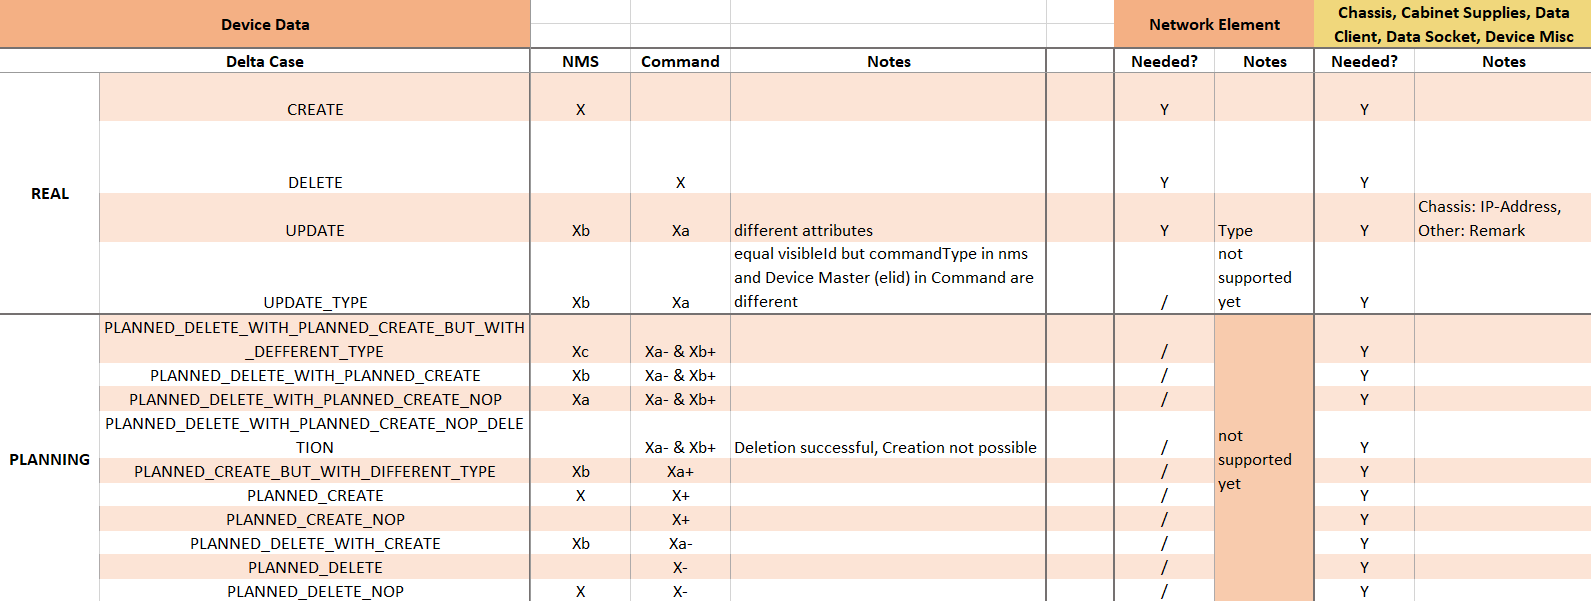
\includegraphics[width=.9\textheight, keepaspectratio, angle=90]{test-data-matrix.png}
    \caption[]{Ausschnitt der Testdatenmatrix, genauer aus der Teilmatrix \enquote{Device Data}}
\end{figure}

\newpage
\section*{C. Ausschnitt eines Rückgabewerts in der \ac{BGW}-Dokumentation}\label{app:bgeDoku}
\begin{lstlisting}[language=json, basicstyle=\scriptsize\ttfamily]
    {
        "id": "placeInZone",
        "type": "CREATE",
        "name": "Place in zone",
        "description": "Place in zone",
        "rest": {
          "definition": {
            "url": "/axis/api/rest/definition/entity/chassis/operation/placeInZone"
          },
          "service": {
            "url": "/axis/api/rest/entity/chassis/placeInZone",
            "method": "post",
            "responseFormats": "JSON"
          }
        },
        "attributes": [],
        "returnAttributes": [],
        "subOperations": [
          {
            "id": "createLinkDeviceMaster",
            "cardinality": "1",
            "relationDefinition": "deviceMaster",
            "type": "CREATE",
            "name": "Create link to Device master",
            "description": "Creates a link to the target entity Device master",
            "rest": {
              "definition": {
                "url": "/axis/api/rest/definition/entity/chassis/operation/placeInZone/suboperation/createLinkDeviceMaster"
              }
            },
            "attributes": [
              {
                "id": "linkedElid",
                "name": "Key Device master (Target)",
                "key": true,
                "nullable": false,
                "required": true,
                "dataType": "STRING",
                "dataLength": 14,
                "preDecimalPlaces": -1,
                "decimalPlaces": -1
              }
            ],
            "returnAttributes": []
          },
          ...
        ],
        ...
    }
\end{lstlisting}

\newpage
\section*{D. Ausschnitt aus dem Konzept zur Testdatengenerierung von Telco-Entitäten}\label{app:telcoKonzept}
Die nächsten drei Seiten sind ein Ausschnitt aus dem PDF-Dokument, welches das schriftliche Konzept für die automatische Testdatengenerierung von Telco-Entitäten darstellt. Konkret behandelt der Ausschnitt die Telco-Entität Bearer. Die Abkürzung \enquote{NE} bezeichnet hierbei ein Objekt der Entität Network Element.
\includepdf[pages={10,11,12}]{files/TDG_Concept_Telco.pdf}
	
\end{document}
